\pagestyle{ayllon}
\label{ayllon}

\pagebreak

\begin{center}
\hspace*{-3.6cm}\raisebox{5cm}{\rotatebox[origin=t]{90}{\huge\textbf{Lançamento}}}
\hspace*{3.1cm}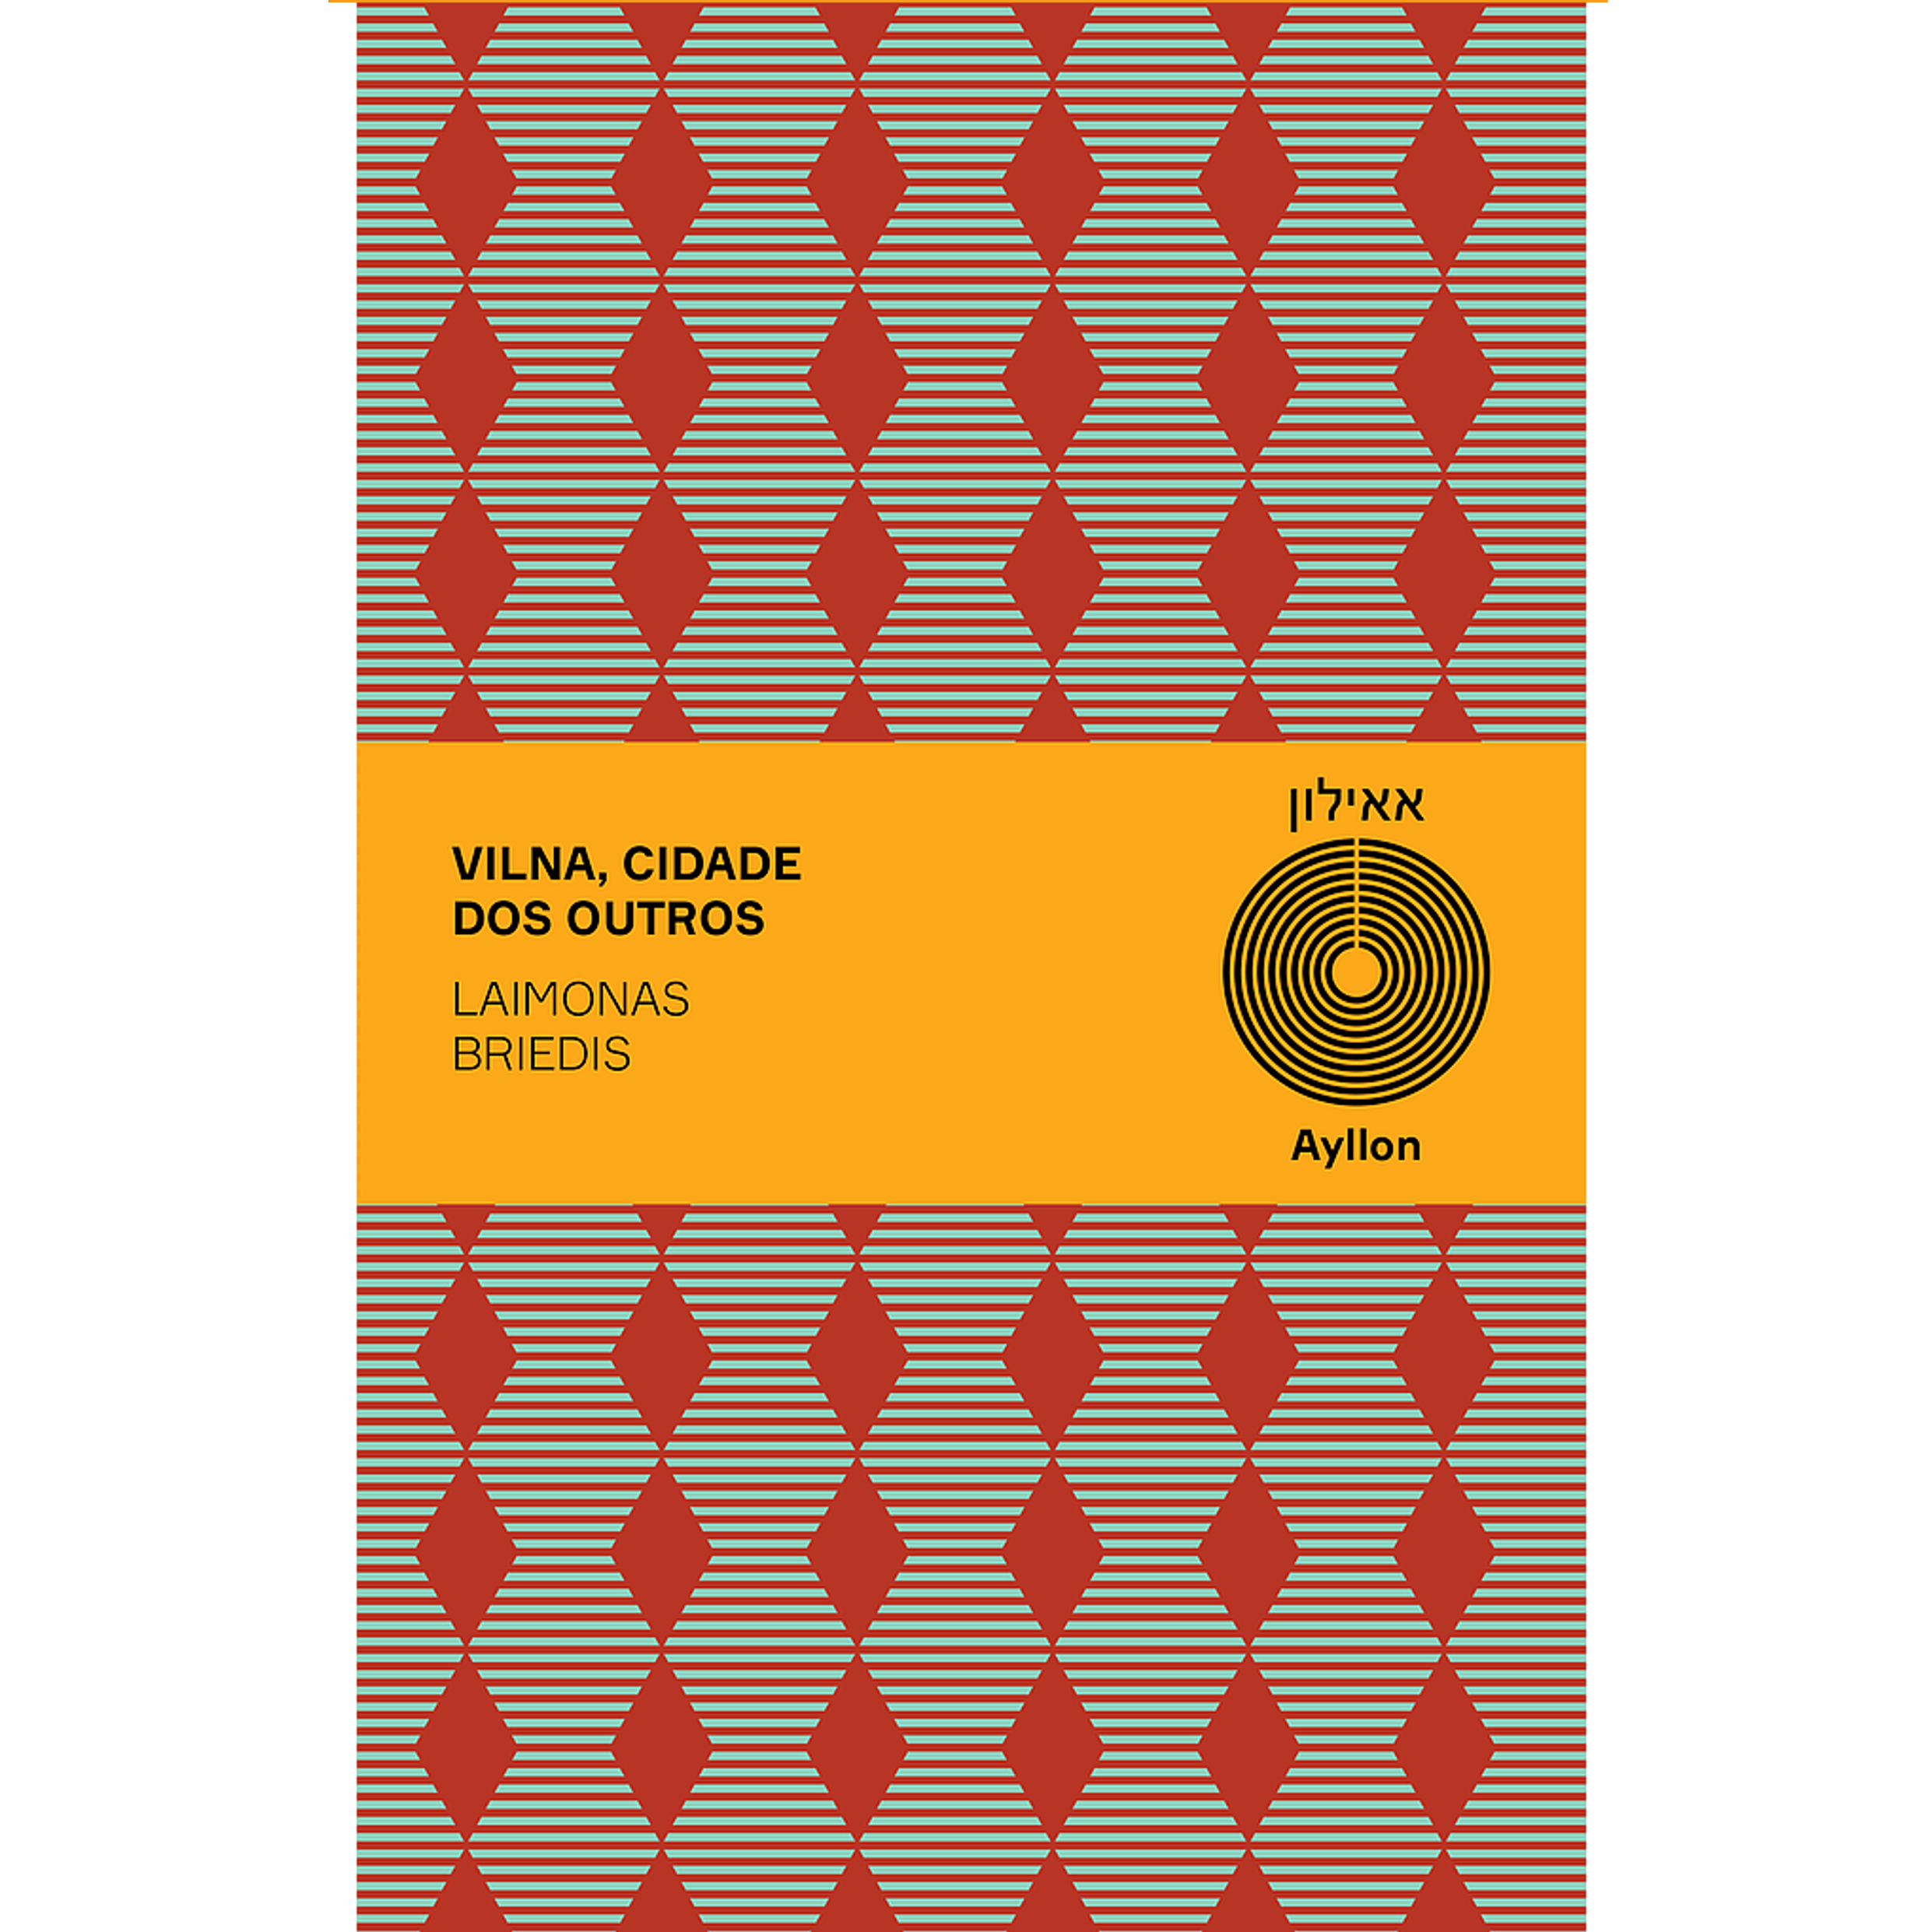
\includegraphics[width=74mm]{./CAPAS/vilna.jpg}
\end{center}

\hspace*{-7cm}\hrulefill\hspace*{-7cm}

\medskip

\noindent{}\textit{Vilna, cidade dos outros} é uma narrativa sobre a capital da Lituânia. \hlc{Escrita com base na cartografia histórica e geografia humana local, a cidade que também foi conhecida como "a Jerusalém da Lituânia" abrigou ao longo dos tempos inúmeros povos, falantes de diversos idiomas, em uma miscelânia cultural: judeus, poloneses, lituanos, ucranianos, bielorussos, russos, alemães, letões, armênios, tártaros e outros grupos minoritários}. Impregnada dentre seus vários componentes pelo barroco, que esteve no limiar da Europa e no contexto de suas mudanças, a cosmopolita cidade também é apresentada através de textos de pessoas ilustres ou desconhecidas, de muitas procedências e línguas, que viveram ou passaram por ela, através de relatos de experiências, sensibilidades e perspectivas próprias.

\vfill

\hspace*{-.4cm}\begin{minipage}[c]{1\linewidth}
\small\textbf{
\hspace*{-.1cm}Editora: Ayllon\\
Título: Vilna, cidade dos outros\\
Autor: Laimonas Briedis\\ 
ISBN: 978-85-77156-65-8\\
Páginas: 380\\
Formato: 13,3x21\,cm\\
Preço: R\$ 99,00
}
\end{minipage}

\pagebreak

\begin{center}
\hspace*{.5cm}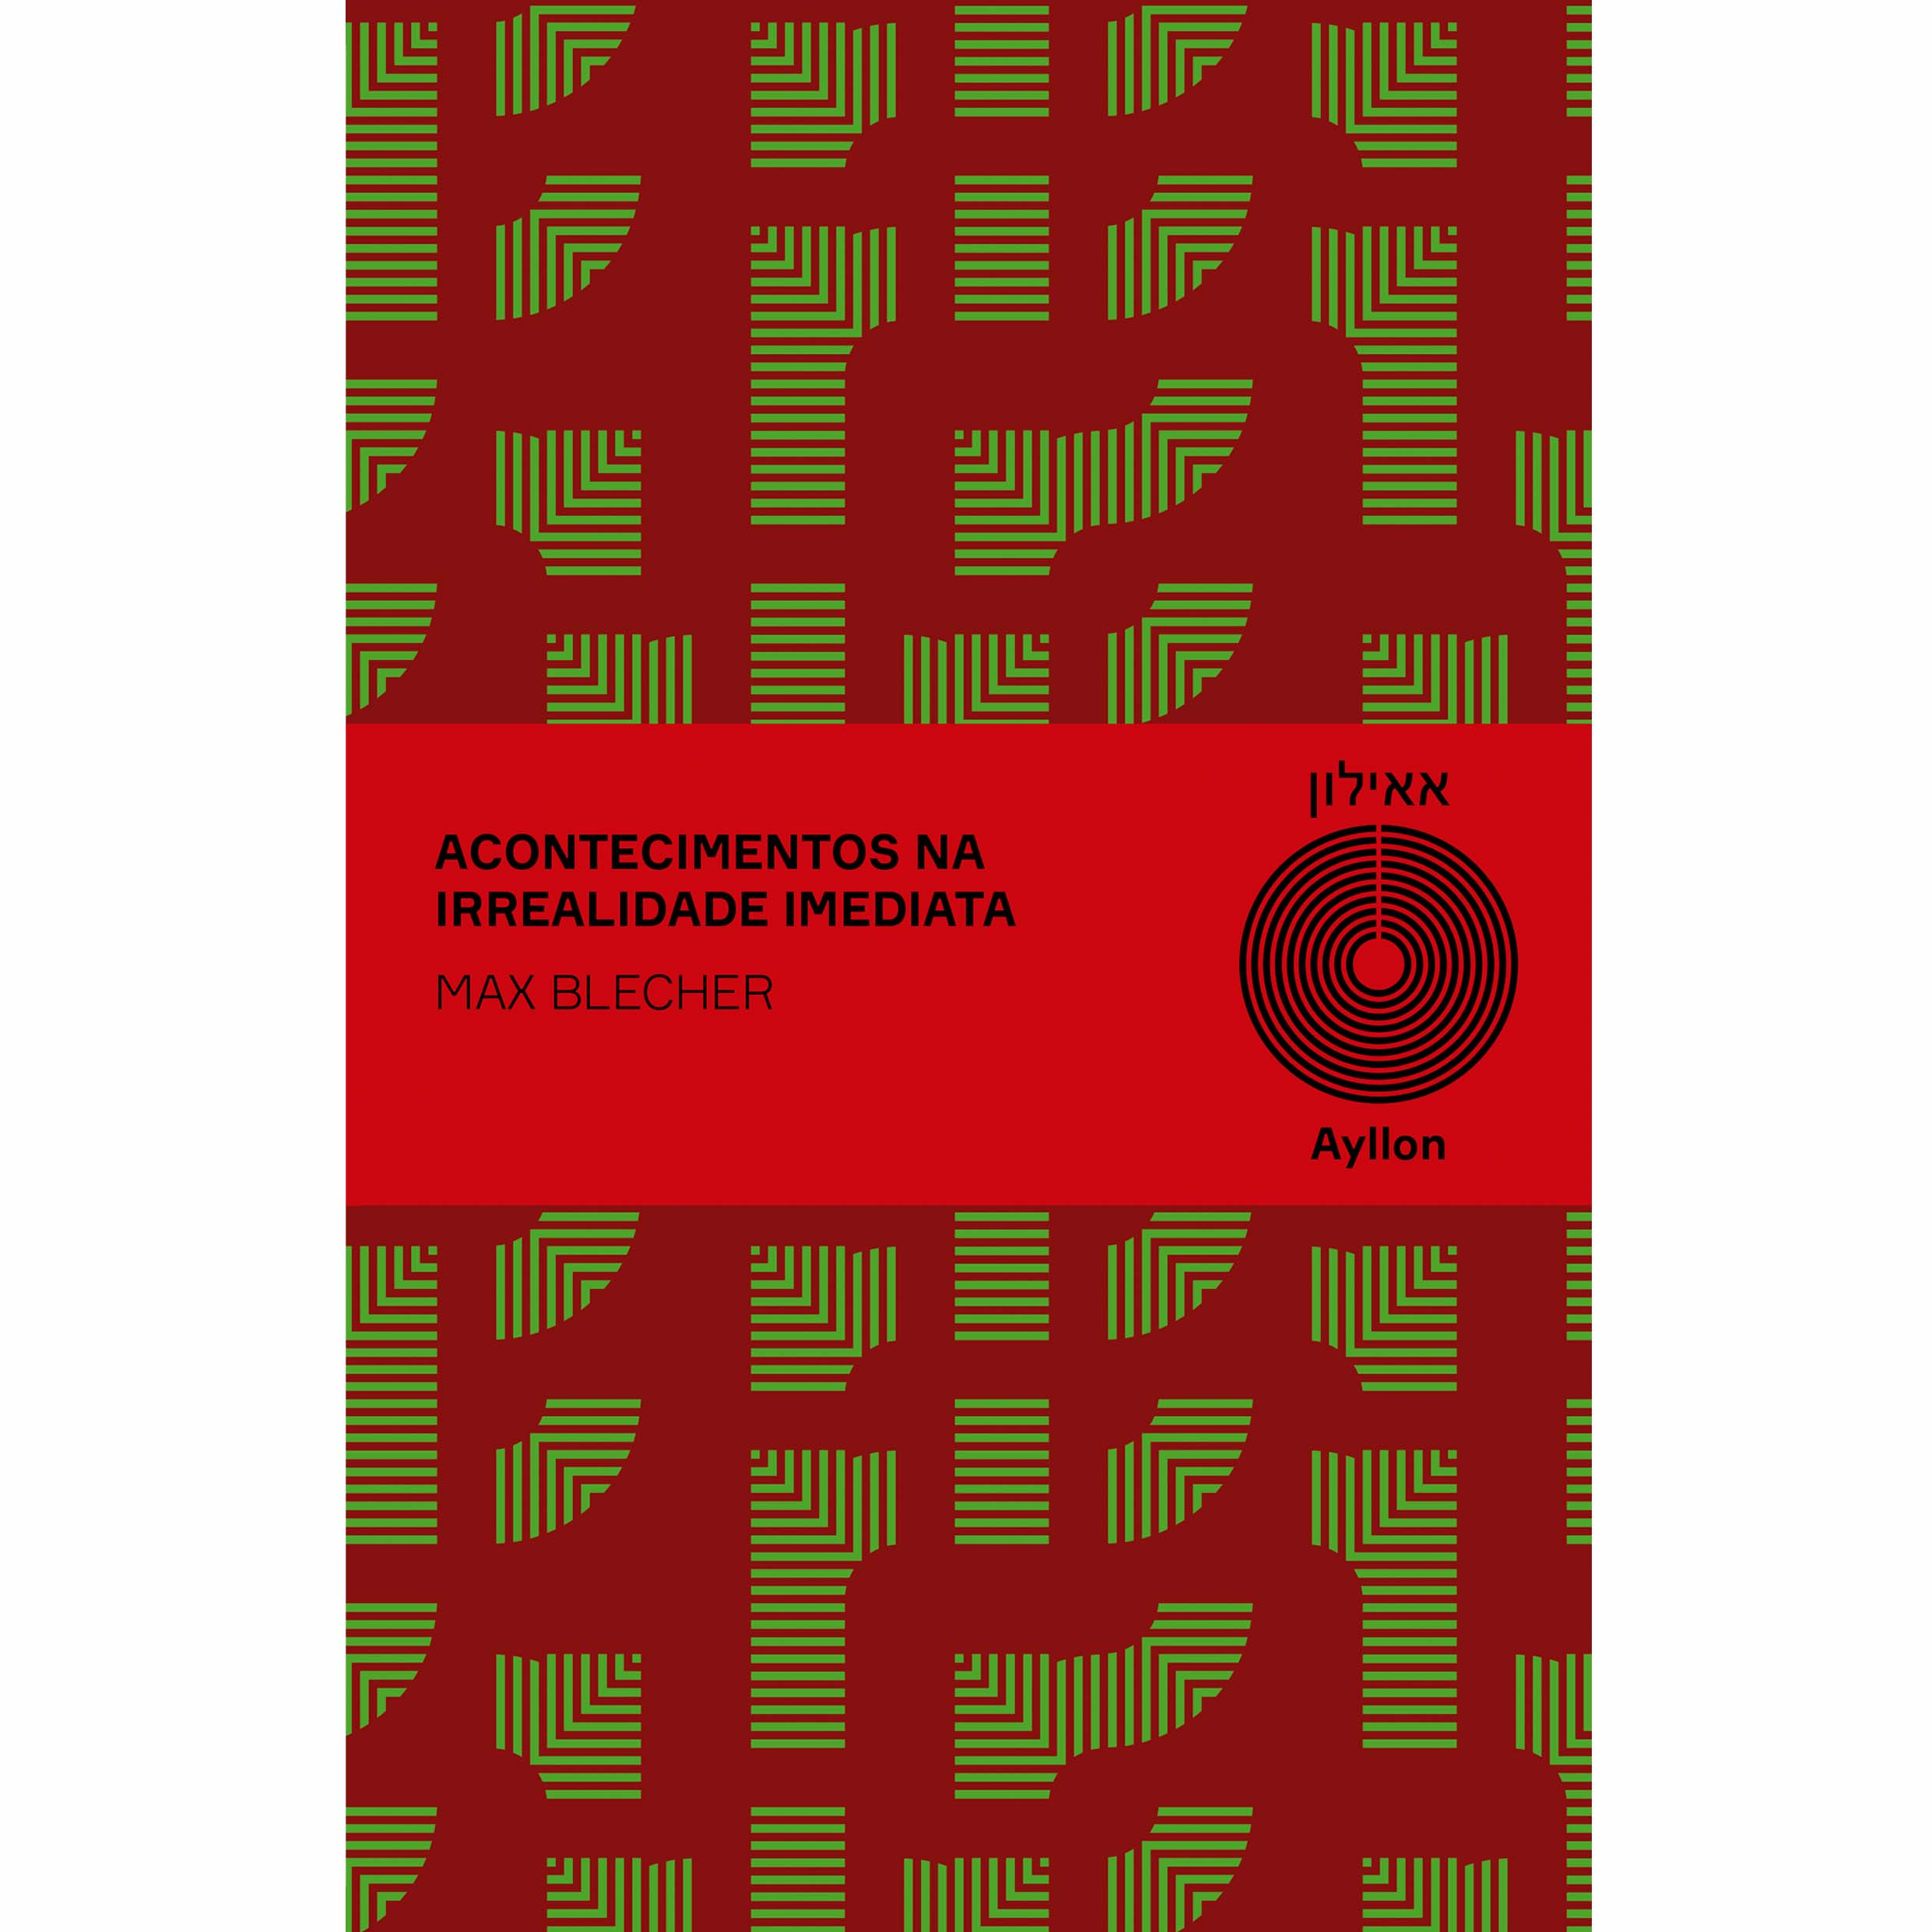
\includegraphics[width=74mm]{./CAPAS/blecher.jpg}
\end{center}

\hspace*{-7cm}\hrulefill\hspace*{-7cm}

\medskip

\noindent{}Uma cidade sem nome, em arrabaldes lamacentos, alamedas abandonadas, grutas, quintais, camarins, interiores ensombrecidos e cômodos semi-habitados com móveis onde repousam objetos cobertos de mofo adquirem uma estranha forma de vida na presença do protagonista.
\textit{Acontecimentos na irrealidade imediata}, de 1936, é um clássico perdido da literatura moderna. Novela do romeno Max Blecher, escrita entre 1930 e 1934, remete a lugares e figuras que marcaram sua juventude. Narra um enigmático conjunto de experiências, as ``crises de realidade'', vertigens que culminam em desmaios momentâneos. O livro se abre com uma dessas crises: `` \hlc{Ao fitar por muito tempo um ponto fixo na parede, às vezes acabo não sabendo mais quem sou nem onde estou. Então, sinto claramente falta da minha identidade, como se eu tivesse me tornado, de repente, um estrangeiro perfeito}. Esse personagem abstrato e minha pessoa real disputam em pé de igualdade minha convicção''.
\vfill

\noindent\begin{minipage}[c]{1\linewidth}
{\small\textbf{
\hspace*{-.1cm}Editora: Ayllon\\
Título: Acontecimentos na irrealidade imediata\\
Autor: Max Blecher\\ 
ISBN: 978-65-89705-07-9\\
Páginas: 170 (provisório)\\
Formato: 13,3x21\,cm\\
Preço: R\$ 54,00\\
}}
\end{minipage}

\pagebreak

\vspace*{1.5cm}

\noindent{}{\nohyphens{\LARGE{Cacilds vidis litro abertis}}}

\bigskip

\hfill{}\scalebox{.8}{MUSSUM IPSUM}

\bigskip
\bigskip
\bigskip

\begin{multicols}{2}
\noindent{}\lipsum[2]

\lipsum[4]

\lipsum[6]


{\small\fakereceipt{
\noindent{}\lipsum[7]
}}

\vspace{\baselineskip}


\lipsum[2]

\lipsum[4]

\lipsum[6]



\noindent{}\textcolor{gray}{\footnotesize\slsc{Trecho de  “O livro dos mandamentos”.}}
\end{multicols}
